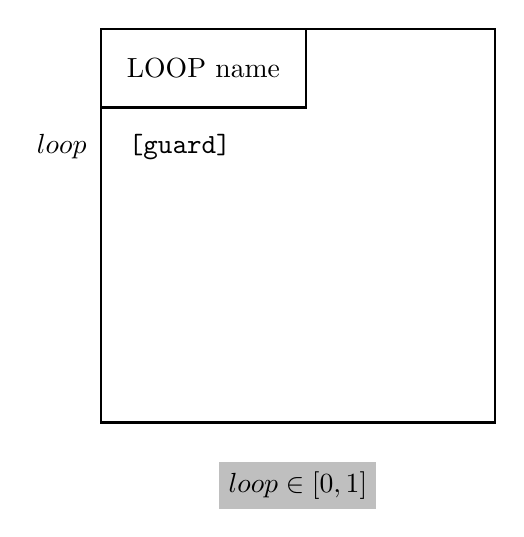
\begin{tikzpicture}[thick]
%%%%%%%%%%%%%%%%%%%%%%%%%%%%%%%%%%%%%%%%%%% HELP LINES
%\draw[help lines] (0,0) grid +(10,10);

%%%%%%%%%%%%%%%%%%%%%%%%%%%%%%%%%%%%%%%%%%% elements
\draw (1,0) rectangle +(5,5);
\node[shape=rectangle, draw=none](p1) at (0.5,3.5){$loop$};
%\draw (1,2) rectangle +(5,1);
%\draw (1,3) rectangle +(5,2);
%\draw (1,5) rectangle +(5,2);


%%%%% guards and constraints
\node[shape=rectangle, draw=black, minimum height=1cm, minimum width=2.6cm](alt)at(2.3,4.5){LOOP name};
\node[shape=rectangle, draw=none](guard) at (2,3.5) {\texttt{[guard]}};
\node[shape=rectangle, fill=gray!50, draw=none](constraint) at (3.5,-0.8) {$loop \in [0,1]$};
\end{tikzpicture}
